\documentclass[12pt]{article}
\usepackage{graphicx}
%\usepackage{wrapfig}
\usepackage{url,hyperref}
\usepackage{fancyhdr}
\pagestyle{fancy}
\title{Artificial Intellegence}
\date{23 January 2020}
\makeatletter
\let\thetitle\@title
\let\theauthor\@author
\let\thedate\@date
%\makeatother

\begin{document}

\begin{titlepage}
     \begin{center}
     
     \begin{large}
     
     \textbf{BANGABANDHU SHEIKH MUJIBUR RAHMAN}\\ \textbf{SCIENCE AND TECHNOLOGY UNIVERSITY}\\
     \textbf{Sheikh Hasina Institute of ICT}
     
     \end{large}
     
     %ADD LOGO
     \\[1in]
     
\includegraphics[width=0.35\textwidth]{Image/logo.png}
     \\[0.5in]
     
     %TOPIC
     \begin{LARGE}
     \begin{tabular}{| c |}
     \hline
     \textbf{LaTex Lab Report on Artificial Intelligence}\\
     \hline
     \end{tabular}
     \end{LARGE}
     
     \\[0.5in]
    
     \begin{flushleft}
     \textbf{ Course Code: CSE156\\}
     \textbf{ Course Title: Technical Writing and Presentation\\}
     \textbf{ Date of submission: \today\\}
     \end{flushleft}
     
     \renewcommand{\tabcolsep}{1pt}
     \begin{tabular}{ | p{7cm} | p{7cm}|} 
     \hline \textbf{Submitted By} & \textbf{Submitted To}\\ 
     \hline
     \textbf{Name: }  Israt Jahan Reshma & \\
     \textbf{ID No: }18ICTCSE041  &     \\
     \textbf{Year: }  First        &   \textbf{Mr. Nasif Ahmed}\\
     \textbf{Semester: }  Second     &    \\
     \textbf{Session: }  2018 - 19  &     Lecturer\\
     \textbf{Department of CSE BSMRSTU(SHIICT)} & \textbf{Department  of CSE BSMRSTU(SHIICT)}\\
     \hline
    \end{tabular}
    
     \end{center} 
\end{titlepage}

%CONTENT PAGE 
    \newpage
    \tableofcontents
	%\rule{\linewidth}{0.2 cm} \\[1.5 cm]
    \newpage
\Huge\section{Introduction} 
\huge \subsection{Fact Follows Fiction:}\large\flushleft As far back as the ancient Greek civilization, people have imagined machines and mechanical men that could work and think like any human. One Greek myth, for example, tells of the Greek god Hephaestus, who built mechanical men to forge powerful weapons and spectacular jewelry. When the king of Crete requested that he make a giant man to guard his island, Hephaestus constructed the metallic warrior Talos. Talos patrolled the shores of Crete until Jason and the Argonauts defeated it.\\
\begin{figure}[h]
\center
  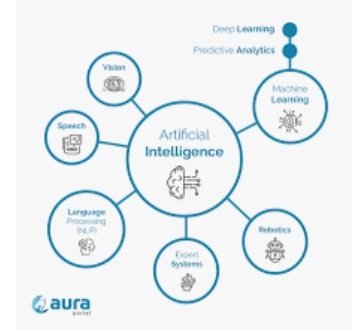
\includegraphics[width=4cm]{Image/IMG_20200125_232757.jpg}
  \caption{}
 
\end{figure}
 In the late 1800s, as the genre of science fiction developed, books about intelligent machines serving human masters sparked the public’s imagination, but not until the 1920s did such machines acquire the name robot. In 1920 Czech playwright Karel Capek published the play R.U.R. (Rossum’s Universal Robots) in which the character Professor Rossum manufactures artificial men to do all the menial chores, called robota in the Czech language. Rossum’s plan backfires and armies of robots are purchased by warring nations. Eventually the robots themselves revolt and attempt to take over all of humankind.\\ 
 In the 1950s and 1960s a series of movies and books portrayed the blessings but more often the horrors of intelligent machines, which took all forms. Some were Talos-like robots made of shiny metal, like Gort in The Day the Earth Stood Still (1951); others were intelligent supercomputers that threatened to take over the world in movies like Colossus: The Forbin Project (1969). In this film the supercomputer that ran the U.S. national defense systems overrode all human control. But perhaps the most famous malevolent supercomputer was HAL 9000, the sinister manager of the spaceship Discovery in 2001: A Space Odyssey (1968). HAL could learn and act independent of human input and in so doing it killed all but one crew member.\\
 
Not all robots or supercomputers have been portrayed as evil. In the 1970s moviegoers fell in love with the flighty C-3PO and quirky trashcan-shaped R2-D2 in the Star Wars series. Without the help of these autonomous beings, the heroes would not have prevailed over the evil empire. And in 2001 audiences connected with the boy robot in Steven Spielberg’s film AI when he expresses emotions and feelings of love toward his adoptive human parents.\\
 These fictional stories reflect humans’ dreams and fears about intelligent machines. And there is an odd correlation between science fiction and science fact. Writers have envisioned worlds that are technologically several steps ahead of reality. They imagined robots on Mars long before the first moon landing and portable minicomputers long before the invention of laptops. Scientists who work in the field of artificial intelligence (AI), the study of intelligent machines, also foresee a future filled with independent, thinking robots and computer companions. Unlike fiction writers, however, they face the daunting challenge of making their dreams a reality. Each year AI researchers come closer to realizing their dreams with new developments in computer programming and robotic engineering.\\ 
\huge\subsection{Real-life AI}
\large\flushleft
 As in fictional stories, the pursuit of intelligent machines has taken two forms. Researchers have created robotic bodies—like that of C-3PO—that look and move like a human. They have even created artificial material similar to human skin that will mask the computer chips and wiring inside a robot’s head. Other researchers are working on robots that learn from experience—like those in Isaac Asimov’s classic story I, Robot—and can express emotions like the robotic boy in director Steven Spielberg’s feature film AI.\\
Fact Follows Fiction 11
The second form of intelligent machines is the allknowing and all-powerful “beings without bodies” like HAL. Artificial intelligence experts have already created supercomputers that navigate and control the space shuttles; other computer systems are powerful enough to effectively run major companies. But AI is not just reserved for grand space exploration or high finance. In fact, much of a person’s daily life is affected by some form of artificial intelligence. AI computer programs keep track of a person’s banking, translate foreign languages, locate a car’s position, and put once hard-to-find information at a person’s fingertips with the Internet. Each year smart machines become more proficient at chores we used to do for ourselves, and people purchase the newest electronic AI gadgets in hopes of making their lives easier. But what happens to a society that gives more and more control to machines? Will fact follow fiction? Will people enjoy a life of friendly companionship with robots like R2-D2 and live blissfully by relying on all-knowing machines to help them get through their days?\\
 Anyone who has been beaten by a computer at a game of chess knows the unsettling feeling of dealing with an intelligent system. Will that unease grow? And as more jobs are given to computers, how will that change humanity? Will people lose skills like remembering phone numbers or calculating large sums? Will people become slaves to the very machines they have created and lose their humanity in a world of mechanization? Will the fictional cautionary tales be heeded, or will the future hold a wondrous collaboration between man and machine? Only time will tell as scientists continue to forge ahead and attempt to make real the amazing dreams of fiction writers.\\
 %\newpage
\Huge
%\center{CHAPTER 2}\\
%\color{blue}
\section{The First Thinking Machines}
\center
\large\flushleft
Gaak was missing. No one knew what it was thinking or if it was thinking at all. The only thing that robotics expert Noel Sharkey knew was that the small robotic unit he had just repaired had disappeared. Gaak had been injured in battle during a “survival of the fittest” demonstration at the Living Robots exhibition in Rotherham, England, in 2002. In this contest predator robots sought out prey robots to drain their energy, and prey robots had to learn to avoid capture or be inactivated.\\
 Gaak, a predator robot, may have had enough of the competition. Only fifteen minutes after Sharkey left the robot’s side, the autonomous machine forced its way out of its corral, sidled past hundreds of spectators, maneuvered down an exit ramp, and left the building. Gaak’s bid for freedom was stopped short when it was almost run over by a car as it fled toward the exit gate.
\begin{figure}[h]
\center
  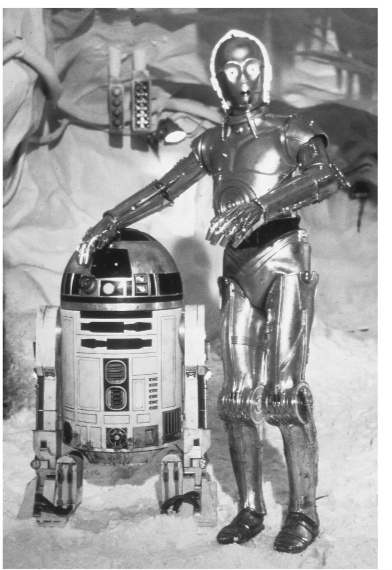
\includegraphics[width=4cm]{Image/IMG_20200125_232951.jpg}
  \caption{}
 
\end{figure}
 Although this may sound like another sci-fi nightmare, it is actually an example of artificial intelligence at work today. AI is the study and creation of machines that can perform tasks that would require intelligence if a human were to do the same job. This emerging and constantly changing field combines computer programming, robotics engineering, mathematics, neurology, and even psychology. As a blend of many sciences, AI has a scattered history. It has almost as
many processes as there are researchers active in the field. Like the limbs of a tree, each new idea spawns another, and the science of artificial intelligence has many branches. But its roots were planted by scientists and mathematicians who could imagine all the possibilities and who created amazing machines that startled the world.\\
\huge
\subsection{The Turing Machine}
\large
 The next and perhaps most influential machine to mark the development of AI was, once again, never even built. It was a theoretical machine, an idea that existed only on paper. Devised by the brilliant British theoretical mathematician Alan Turing in 1936, this simple machine consisted of a program, a data storage device (or memory), and a step-by-step method of computation. The mechanism would pass a long thin tape of paper, like that in a ticker-tape machine, through a processing head that would read the infor
16 Artificial Intelligence
mation. This apparatus would be able to move the paper along, read a series of symbols, and produce calculations based on the input on the tape. The so-called universal computer, or Turing machine, became the ideal model for scores of other researchers who eventually developed the modern digital computer. Less than ten years later, the three most powerful nations in the world had working computers that played an integral part in World War II.\\
\huge
\subsection{The Binary Code}
\large 
ENIAC and all other computers that have followed have spoken the same basic language: the binary code. This is a system of symbols used to program a computer. Proposed by U.S. mathematician Claude Shannon and expanded on by Hungarian-born mathematician John von Neumann in the 1940s, the binary code is a language with only two symbols, 0 and 1. Shannon and von Neumann showed that the simplest instruction was yes/no, or the flicking on and off of a switch, and that any logical task could be broken down to this switching network of two symbols. The system is binary, based on two digits, and combinations of these two digits, or bits, represent all other numbers.Inside the computer,electrical circuits operate as switches.
\begin{figure}[h]
\center
  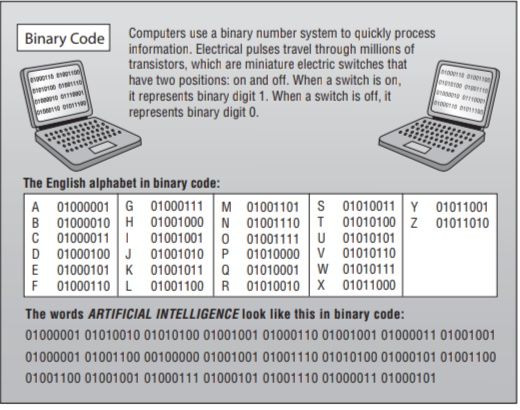
\includegraphics[width=5cm]{Image/IMG_20200125_233115.jpg}
  \caption{}
 \end{figure}
  When a switch is on, it represents the binary digit 1. When a switch is off, it represents the binary digit 0. This type of calculation is fast and can be manipulated to count, add, subtract, multiply, divide, compare, list, or rearrange according to the program. This simple digital system can be used to program a computer to do even the most complex tasks. The results of electrical circuits manipulating strings of binary digits are then translated into letters or numbers that people can understand. For instance, the letter A is represented by the binary number 01000001. Today, by reading and changing binary digits, a machine can display a Shakespearean sonnet, play a Mozart melody, run a blockbuster movie, and even represent the entire sequence of human DNA.\\
 
\Huge
\subsection {\textbf {Smaller and Faster}}
\large
The basic digital language of early computers was fast, but the hardware that performed the tasks was not. Vacuum tubes were unreliable and broke down frequently. Computing was made faster with transistors, a crucial invention developed in the 1950s. A transistor is a miniature electronic switch that has two operating positions: on and off. It is the basic building block of a computer that enables it to process information. Transistors are made from silicon, a type of material that is called a semiconductor because certain impurities introduced to the silicon affect how an electrical current flows through it. These early transistors were lighter, more durable, and longer lasting. They required less energy and did not attract moths, as ENIAC’s vacuum tubes did. They were also smaller, about the size of a man’s thumb. And smaller translated to faster. The shorter the distance the electronic signal traveled, the faster the calculation. The next improvement came with the invention of the integrated circuit, an arrangement of tiny transistors on a sliver, or chip, of silicon that dramatically reduced the distance traveled.
\newpage
\Huge
\section{\textbf{Mind Versus Metal }}
\center
\large\flushleft
The activities that kindergarten-age children perform effortlessly, like knowing the difference between a cup and a chair, or walking from one room to the next without bumping into the wall, were not thought of as intelligent behavior or worthy of study by traditional AI researchers. But when traditional systems did not perform as they had expected, experts in AI began to wonder what intelligence really meant. They also began to think about different ways to show intelligence in a machine. Although the definition of intelligence is still debated today, scientists understand that intelligence is more than the sum of facts a person knows; it also derives from what a person experiences and how a person perceives the world around him or her. Neil Gershenfeld, author of When Things Start to Think, believes that “we need all of our senses to make sense of the world, and so do computers.”5 As ideas about human intelligence changed, so did approaches to creating artificial intelligence.\\
 In the 1980s AI experts working in robotics began to realize that the simple activities humans take for granted are much more difficult to replicate in a machine than anyone thought. As expert AI researcher Stewart Wilson of the Roland Institute in Cambridge explains:\\
AI projects were masterpieces of programming that dealt with various fragments of human intelligence. . . . But they were too specialized. . . . They couldn’t take raw input from the world
around them; they had to sit there waiting for a human to hand them symbols, and they then manipulated the symbols without knowing what they meant. None of these programs could learn from or adapt to the world around them. Even the simplest animals can do these things, but they had been completely ignored by AI.\\
\Huge
\subsection{\textbf{Insect Intelligence }}
\large
 Brooks started at the bottom of the evolutionary ladder, with insects, which were already capable of doing what the most sophisticated AI machines could not do. Insects can move at speeds of a meter or more per second, avoid obstacles in their path, evade predators, and seek out mates and food without having to have a mental map as Shakey the robot did. Instead of preprogramming behaviors, Brooks programmed in less information, just enough to enable his AI robots to adapt to objects in their path. He felt that navigation and perception were key to mastering higher-level intelligence. This trend became known as the bottomup approach, in contrast to the top-down approach of programming in all necessary information.\\
 \Huge
\subsection{\textbf{ How the Brain Works}}
\large
 \begin{figure}[h]
\center
  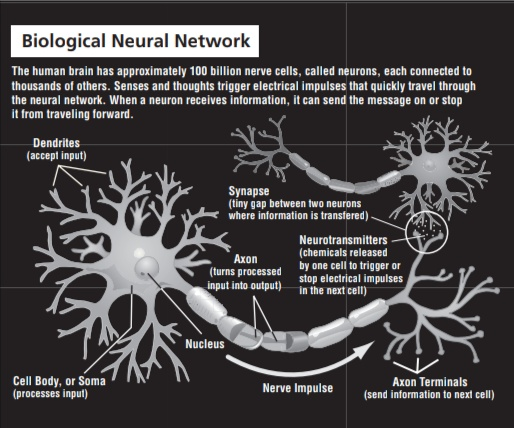
\includegraphics[width=5cm]{Image/IMG_20200125_233520.jpg}
  \caption{}
 \end{figure}
 \large
 The human brain has close to 100 billion nerve cells, called neurons. Each neuron is connected to thousands of others, creating a neural network that shuttles information in the form of stimuli, in and out of the brain constantly.\\
 Each neuron is made up of four main parts: the synapses, soma, axon, and dendrites. The soma is the
30 Artificial Intelligence
body of the cell where the information is processed. Each neuron has long, thin nerve fibers called dendrites that bring information in and even longer fibers called axons that send information away. The neuron receives information in the form of electrical signals from neighboring neurons across one of thousands of synapses, small gaps that separate two neurons and act as input channels.\\
Once a neuron has received this charge it triggers either a “go” signal that allows the message to be passed to the next neuron or a “stop” signal that prevents the message from being forwarded. When a person thinks of something, sees an image, or smells a scent, that mental process or sensory stimulus excites a neuron, which fires an electrical pulse that shoots
Mind Versus Metal 31
Dendrites (accept input)
Nucleus
Axon Terminals (send information to next cell) 
Axon (turns processed input into output) 
Cell Body, or Soma (processes input) Nerve Impulse
Synapse (tiny gap between two neurons where information is transfered)
Neurotransmitters (chemicals released by one cell to trigger or stop electrical impulses in the next cell)
The human brain has approximately 100 billion nerve cells, called neurons, each connected to
 thousands of others. . Biological Neural Network
out through the axons and fires across the synapse. If enough input is received at the same time, the neuron is activated to send out a signal to be picked up by the next neuron’s dendrites. Most of the brain consists of the “wiring” between the neurons, which makes up one thousand trillion connections. If these fibers were real wire, they would measure out to an estimated 63,140 miles inside the average skull. \\
 Learning comes when patterns are strengthened, but if connections are not stimulated, they are weakened. For example, the more a student repeats the number to open a combination lock, the more the connections that take in that information are bolstered to create a stronger memory that will be easily retrieved the next time. At the end of the school year, when a student puts the lock away, that number will not be used for a couple of months. Those three numbers will be much harder to recall when fall comes and that student needs to open the lock again. \\
\newpage
\Huge
\section{\textbf{Everyday AI }}
\center
\large\flushleft
The real success of AI is that most people are simply unaware of how significantly it affects and enables the routines of daily life. A man gets up in the morning to the smell of coffee already brewing. This is thanks to a microchip inside the coffee machine that allows him to program his coffeemaker to turn itself on while he is still sleeping. Another microchip keeps his toast from burning and remembers which setting from light to dark he likes best. At one time these were all novel forms of AI.  \\
\begin{figure}[h]
\center
  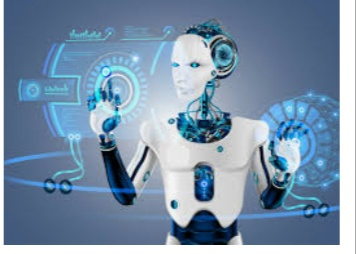
\includegraphics[width=5cm]{Image/IMG_20200125_232725.jpg}
  \caption{}
 \end{figure}
Already there are ovens on the market that keep food chilled until it starts to cook at a preset time. There are refrigerators with Web pads embedded in the doors to display recipes or to surf the Internet. The company iRobot now manufactures a robotic vacuum cleaner that buzzes around a room without a human operator. But AI in the home today offers just a glimpse of what future household appliances will look like. “Most people don’t realize fundamental changes in kitchen gear are coming. But in a decade or so, they won’t know how they lived without their e-kitchens,” \\
\huge
\subsection{Computer Games}
\large
Traditionally, AI computer programs have worked in the background, making sure that the digital environment of forests, smoking volcanoes, and rambling paths run smoothly. But AI is also used to make computer games more challenging for their human participants. Most games are rule-based, which means that the computerized characters such as enemy guards, friendly wingmen, or monsters follow a basic set of rules according to what is happening around them. For example, if an enemy guard encounters a monster, it will attack the creature. If the creature flees, the enemy guard will chase after it, and if the enemy guard is fired on, it will dodge the bullet, spear, or laser ray. But these behaviors can become predictable for an experienced human player. All of the criteria do not have to be present for a character to act. There is flexibility in its behavior responses.  \\
\huge
\subsection{Driving AI}
\large
After seeing a movie, a family may hop into the car and again be confronted with more applications of AI at work. Electronic sensors throughout the car’s engine monitor its efficiency. A neural network computer chip in newer models reduces the car’s emissions and improves fuel efficiency by monitoring fuel combustion. Designed by the National Aeronautics and Space Administration’s (NASA’s) Jet Propulsion Laboratory, the chip can learn how to diagnose misfiring faster and alert the driver to engine problems.\\
\huge
\subsection{E-commerece}
\large
Today a person does not have to get into a car to go shopping, thanks to sophisticated AI applications and the Internet. In 1995 almost no businesses conducted their affairs over the Internet. But by the year 2003 business-to-consumer sales on the Internet exceeded \$100 billion and business-to-business sales more than \$3 trillion.\\ 
\huge
\subsection{AI in Business}
\large
 AI is not just found in ecommerce. Expert systems help run most of the major businesses the world over. Wal-Mart harnesses an expert system enhanced with an ANN to sift through the data of all the sales at more than three thousand stores to find patterns and relationships between stores, products, and customers. It can find the pattern in what sells and what does not faster than hundreds of human analysts can. Expert systems even manage billions of dollars in the stock market.\\
 \huge
 \subsection{The Digital Doctor}
 \large
  Expert systems are also used in medicine to help doctors diagnose patients. In a 1997 study researchers concluded that medical students learn more than 47,000 facts and 29,000 concepts in just the first two years of medical school. Ideally all of that knowledge can be programmed into an expert system.\\
\newpage
\Huge

\section{\textbf{AI and Robotics}}
\center
\large\flushleft 
In 1958 Joseph Engelberger created the first robots— called Unimates—for factory work. They looked nothing like the fictional robots in movies or books; they looked more like giant flexing arms. The robots were hydraulically powered and programmed to move in a repeated pattern with exacting precision. Automobile manufacturers soon replaced assembly line workers with Unimates, which could perform the most exacting and physically demanding tasks.\\
A person who picks up a hammer and pounds in a nail does not think about the distance between his hand and the hammer or what force is needed. That mathematical and geometric calculation is immediate and unconscious. But that process must be hardwired into industrial robot computers so that mechanical movements are precise.\\
\begin{figure}[h]
\center
  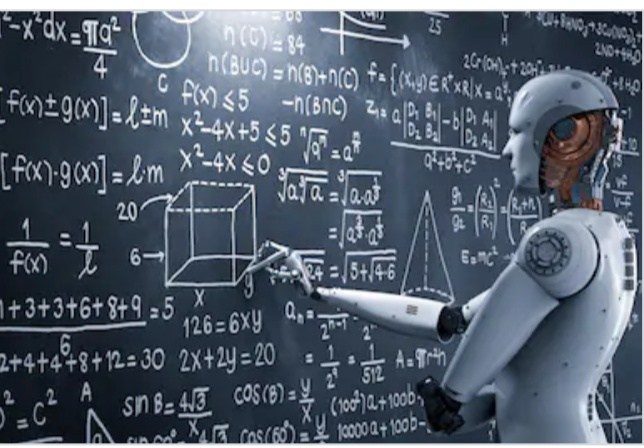
\includegraphics[width=5cm]{Image/IMG_20200125_232848.jpg}
  \caption{}
 \end{figure}
These giant arms are dangerous machines that swivel, swing, hammer, and weld with great force as partially assembled cars move past them. The welding arm must create strong, perfect seams to connect large metal panels on the assembly line. First it must analyze the alignment with its laser vision system. If it detects a misalignment, the robotic arm adjusts the pieces so that they line up correctly. Then it welds them to create the strongest bond possible. This kind of repetitive and precise work is perfectly suited for an AI machine that does not cough, sneeze, blink, or get tired and make a mistake during welding. \\
\huge

\subsection{Robot Explorers} 
\large
Why mimic nature? Researchers hope these designs will be able to go where humans cannot go and do what humans cannot do. Robots do not need oxygen to breathe; they do not get claustrophobic or feel pain. Crab robots can blend into the seabed and patrol underwater for hours. The military hopes they can be used for detecting underwater mines. Insectoid robots can crawl into the tiniest spaces, like into small pipes or inside a wall, and snakebots can slither into cracks and crevices. But not all robotic explorers look like animals. Some resemble tiny tanks or golf carts.\\
\huge
\subsection{Search-and-Rescue Robots}
\large
When the twin towers of the World Trade Center were destroyed on September 11, 2001, robotics expert Robin Murphy and three colleagues from the University of South Florida drove eighteen hours to New York City to help search through the rubble for survivors. They brought eight different search-and-rescue robots with them. The most successful was a miniature tank with treads that crawled into voids thirty feet deep. Although the robots did not discover any survivors, they did prove their usefulness. \\
 \huge
 \subsection{Warbots}
 \large
  Many search-and-rescue robots and animal robots are products of research and development programs sponsored in part by the U.S. military. The Defense Advanced Research Projects Agency (DARPA) hopes that in the future whole schools of robotic fish will patrol shipping channels looking for sunken mines, and a patrol of Mecho-geckos equipped with cameras and audio equipment can be sent up the side of a skyscraper to peek into windows and assess the situation inside. According to military robotics pioneer Scott D. Myers, “Military robots are being developed and fielded to do three things: perform the dull, the dirty and the dangerous.”\\
 \huge
\subsection{The Race for Unmanned Vehicles}
\large
   In 2001 the U.S. Congress mandated that one-third of military ground vehicles be unmanned by the year 2015. That means they should be able to navigate, steer, and respond to various situations without the help of a driver. The parts needed for such a vehicle are advanced laser, radar, and sonar sensor systems to help the vehicle navigate, and Global Positioning System (GPS) to plot its location. So far all the components have not been assembled to create a workable machine that can maneuver across rocky terrain on its own. One prototype, called Navlab II, is a U.S. Army truck driven by a computer called ALVINN (Autonomous Land Vehicle in a Neural Network).
\newpage
\Huge

\section{\textbf{In Pursuit of the Mechanical Man}}
\large\flushleft 

Robot soldiers in any form may be decades away, but that task is simple compared with the skills and efforts needed to produce a robot that could be mistaken for a real human. Creating a humanoid robot is the ultimate goal for many AI researchers, and the most daunting. A convincing humanoid robot would have to walk, gesture, and maneuver as easily as a human, understand the spoken language, be able to communicate, and perhaps even be able to feel emotions and respond to feelings. These are just some of the challenges that AI researchers in labs all over the world must consider.\\
 The scientific research in pursuit of the mechanical man is scattered. Researchers tend to specialize in only one small area of humanoid robotic operation such as speech recognition, visual perception, or mobility, each of which is a highly technical, complex discipline in itself. This is an enormously costly endeavor with an uncertain timeline. For many years, Japan has led the research in humanoid robotics because, as Hirohisa Hirukawa of Japan’s National Institute of Advanced Industrial Science and Technology says, “We are confident that the long-term future of humanoid robots is bright.”\\
\huge
Why Make It Look Human?\\
\large
 Researchers already know how to make machines that are sturdy enough to be dropped onto another planet, smart enough to run businesses, and precise enough to perform surgery. So why would scientists go to all the trouble of making a robot look like a person? This question is hotly debated. Some scientists believe there is no reason. So far, nonhumanoid robots perform better than those with humanoid designs, and it is less expensive to create machines that maneuver on several legs or on wheels or treads. Some researchers raise ethical concerns that if robots look too human there may be the potential for abuse. “Robots need to be designed so that they will be regarded as appliances rather than as people,”18 says John McCarthy of Stanford University. People may treat humanoid robots as slaves,and that is one relationship that ethicists fear could carry over to interpersonal relationships.\\
 \huge
\subsection{Walk This Way}
 \large
 Walking upright is extremely difficult to duplicate and requires a lot of AI computing power. It requires balance, coordination, muscle power, and flexibility just to take three steps across a smooth tile floor in a straight line. But stepping out into an unfamiliar rocky terrain with many obstacles in a robot’s path requires even more AI power to adjust a step, alter foot placement, and register ground resistance—things people do without conscious thought.\\
  Honda’s robot, ASIMO (Advanced Step in Innovative Mobility), is able to walk backward and sideways, go up and down stairs, and even play soccer. ASIMO looks like a small child traipsing around in a white plastic space suit. ASIMO is only four feet tall, but it can simulate human locomotion and use its arms in a realistic fashion. Its designers made special efforts to make it cute so that it was not perceived as threatening and would be more easily accepted. In 2003 ASIMO marched into a state dinner attended by the prime ministers of Japan and the Czech Republic. ASIMO shook hands with Prime Minister Vladimir Spidla and placed a bouquet of flowers at the base of a statue honoring science fiction author Karel Capek, who coined the term robot in 1920.\\
  \huge
  \subsection{Getting Around}
  \large
   Being able to move and walk on two legs is one accomplishment, but knowing how to navigate is another. Using preprogrammed maps like Shakey the robot used fifty years ago is no longer the way robots get around. Today genetic algorithms direct robotic navigation and control systems so that a robot can learn and adapt to any new environment. There are many navigation programs under experimentation, but the most unusual uses pain as a navigational tool.\\
   \huge
   \subsection{Sensory Perception}
   \large
    Few robots are equipped to perceive stimuli as pain, but sensory perception is key to making an effective humanoid robot or any other artificial intelligence. Humans experience the world through five senses. In order for a robot to interact with humans effectively, it has to be able to experience what humans experience. Without the senses of hearing, touch, sight, taste, and smell, people would not be able to act fully within their environment. Even Alan Turing felt that perception was important in his early theoretical design. In his paper “Computing Machinery and Intelligence” he suggested, “It is best to provide the machine with the best sense organs that money can buy and then teach it to understand and speak English. This process could follow the normal teaching of a child.”\\
\huge
\subsection{Artificial Vision}
\large
Many aspects of human sensory perception are difficult if not impossible to duplicate. The human eye, for example, is an incredibly complex structure that provides frontal and peripheral vision; a pair of eyes also provides depth perception and better form recognition.  The eyes register the level of light and measure depth and distances of objects. The eyes sift through a lot of information before any encoded messages are sent to the brain, where 60 percent of the cerebral cortex is devoted to processing visual information. Scientists know how the eye operates—the mechanics of the eye and its movements can be duplicated—but scientists know much less about how eye-brain perception works. Duplicating that connection is more difficult.\\
\huge
\subsection{Artificial Ears}
\large
 Like eyes, ears are complex organs. The human ear is capable of registering and identifying thousands of different sounds. A person can determine what made the sound and how far away the source of the sound may have been.  The perception comes in the form of complex AI programs that register sound and match it to a stored catalog of recognizable noises.\\
 \huge
 \subsection{Touch}
 \large
  The sense of touch is also very complicated. Large industrial robotic arms are dangerous when they maneuver with great force; a humanoid robot would need to have a delicate sense of touch so that if it bumped into a person, the robotic arm would recoil automatically without harming the human.\\
  \huge
  \subsection{Educating Cog}
  \large
   A robot that can touch, see, and hear is ready to experience the world as a human does.. A human infant learns through trial and error as it encounters each new aspect of its environment. Each new piece of information it learns is filed away and used as a basis for more experiences and learning opportunities. Cog, created at MIT more than ten years ago, learns the same way but is still no more knowledgeable than a six-month-old baby.\\
   \huge
   \subsection{Emotions}
   \large
    Down the hall from Cog is its cousin, Kismet. Inspired by Cog’s infantile behavior, researcher Cynthia Breazeal created Kismet, one of the most sociable robots. Whereas no one treats the hulkish Cog like a baby, people frequently use baby talk with Kismet. A cartoonish head bolted to a table, Kismet will respond to a person’s approach, waggle its fuzzy, caterpillar-like eyebrows, and turn up its red licorice-whip lips in a grin.\\
 \newpage
\Huge
\section{\textbf{The Future of AI}}
\center
\large\flushleft   
AI of the future may not look like Cog or have the moves of ASIMO, but it will probably exhibit many of the same attributes that are being perfected in these humanoid robots. The science of artificial intelligence is less than sixty years old, which is young for a branch of science, yet AI has advanced phenomenally since the early days of moth-ridden vacuum tubes. The future of AI is hard to predict, but no one questions that it will be more available and more abundant and present in people’s lives. Some experts anticipate that in the future AI hardware will become smaller, AI will become an essential element of caring for the elderly, and it will include a blending of the best of both human and mechanical intelligence.\\
\huge
\subsection{Mini AI}
\large
 The direction of all electronics and technology continues to be toward ever smaller and more portable products. The first generation of computers, giants that filled entire rooms with whirring gears and fans, gave way to desktop versions run by transistors. The technology shrank dramatically with the invention of silicon chips. Laptops have been miniaturized to handheld computers, and cell phones are half the size they were just five years ago. That trend is reflected in AI also.\\
 \huge
 \subsection{Seniorbots}
 \large
  Monitoring health is an increasing concern in the U.S. medical community. Within fifty years, more than 30 percent of the population will be over the age of sixtyfive, and the National Institute on Aging predicts that more than 14 million Americans will be diagnosed with Alzheimer’s disease. With fewer caregivers and a growing population of potential patients, people will need other kinds of assistance to live happier, safer, and more independent lives. \\
  \huge
  \subsection{Cyborg Science}
  \large
   In the movie Star Trek: First Contact, Captain Jean-Luc Picard is captured by a race of creatures called the Borg that are part man and part machine. Picard’s human parts are slowly replaced by wire, metal, and silicon. The idea might seem unsettling for a squeamish moviegoer, but it is exciting to AI researchers and neuroscientists who hope to make bionics a reality—to create not a hostile Borg race that would try to take over the universe but artificial cognitive parts that would be available when a person’s biological parts fail.\\
   \huge
   \subsection{AI Ethics}
   \large
  The interfacing of brain and machines and robots taking care of grandparents are unsettling ideas to some people. Much time, effort, and technology has been, and will continue to be, spent on making machines that are intelligent. But not as much attention has been paid to a code of ethics to guide the use of artificial intelligence. The Internet has already called into question people’s right to privacy and intellectual property rights that protect writers and other creators who show their work online.\\
  Isaac Asimov wrote the Three Laws of Robotics so that humans would always maintain control. Asimov’s fictional robots had superhuman strength and superhuman intelligence, so it was vital to keep that power in check. His three laws stated:\\  1. A robot may not injure a human being, or, through inaction, allow a human being to come to harm.\\
   2. A robot must obey the orders given to it by human beings except when such would conflict with the First Law.\\ 
   3. A robot must protect its own existence as long as such protection does not conflict with the First and Second Laws.\\
   \huge
   \subsection{AI Power}
   \large
    Most people do not realize how much of their lives are affected by AI and cannot imagine how it will expand in the years to come. People surf the Internet with AI search engines and encounter intelligent agents when they buy a product from a Web site. Their bank accounts and credit cards are monitored with AI software, and transportation systems run smoothly with artificial intelligence programs. Every e-mail and every cell phone call is routed using AI networks. The appliances in the kitchen and the car in the driveway all have parts that use artificial intelligence technology. And that is only a small taste of what AI has accomplished in the last sixty years. \\
\newpage
\huge
\center
\textbf
MATHE:\\
\large     
$$x^3+y^3=1$$ 
$$2x^2-y^9=5$$
$$3x^{34}=y^{10}+z^4=1$$
$$2x^{3x^{10}+9}+y^{100}=z^{x+1}$$
$$x_2+x_1=1$$
$$x_{100}+y_{100}=100$$
$$2x_{3x_{10}+9}-z_{x+1}=10$$
$$x_{1_2}$$
sin$\alpha$+sin$\beta$=1\\
area of circle=$\pi$$r^2$\\

\end{document}
